\documentclass[]{beamer}
\mode<presentation>
{
  \usetheme{Warsaw}
  \definecolor{mcgarnet}{rgb}{0.38, 0, 0.08}
  \definecolor{mcgray}{rgb}{0.6, 0.6, 0.6}
  \setbeamercolor{structure}{fg=mcgarnet,bg=mcgray}
  %\setbeamercovered{transparent}
}


\usepackage[english]{babel}
\usepackage[latin1]{inputenc}
\usepackage{times}
\usepackage[T1]{fontenc}
\usepackage{tikz}
\usepackage{graphicx}
\usepackage{fancyvrb}
\usepackage{adjustbox}

\newcommand{\imagesource}[1]{{\centering\hfill\break\hbox{\scriptsize Image Source:\thinspace{\small\itshape #1}}\par}}

\title{10 - How to Eat an Elephant}


\author{Dr. Robert Lowe\\}

\institute[Maryville College] % (optional, but mostly needed)
{
  Division of Mathematics and Computer Science\\
  Maryville College
}

\date[]{}
\subject{}

\pgfdeclareimage[height=0.5cm]{university-logo}{images/Maryville-College}
\logo{\pgfuseimage{university-logo}}



\AtBeginSection[]
{
  \begin{frame}<beamer>{Outline}
    \tableofcontents[currentsection]
  \end{frame}
}


\begin{document}

\begin{frame}
  \titlepage
\end{frame}

\begin{frame}{Outline}
  \tableofcontents
\end{frame}


% Structuring a talk is a difficult task and the following structure
% may not be suitable. Here are some rules that apply for this
% solution: 

% - Exactly two or three sections (other than the summary).
% - At *most* three subsections per section.
% - Talk about 30s to 2min per frame. So there should be between about
%   15 and 30 frames, all told.

% - A conference audience is likely to know very little of what you
%   are going to talk about. So *simplify*!
% - In a 20min talk, getting the main ideas across is hard
%   enough. Leave out details, even if it means being less precise than
%   you think necessary.
% - If you omit details that are vital to the proof/implementation,
%   just say so once. Everybody will be happy with that.

\section{Complexity and Programming}
\begin{frame}{A Bite of Wisdom}
    \begin{block}{}
    There is only one way to eat an elephant: \uncover<2->{a bite at a time.
    \newline\textit{-- Desmond Tutu}}
    \end{block}
\end{frame}

\begin{frame}{Software and Complexity}
    \begin{block}{With Apologies to Douglas Adams}<+->
        Useful software is big!  You just won't believe how vastly, 
        hugely, mind-bogglingly big it is.  I mean, you may think that
        program three is difficult, but that's just peanuts compared
        to real applications.
    \end{block}

    \begin{itemize}[<+->]
        \item A small useful application is usually around 5,000 lines
            of code.
        \item Most real-world software applications have more than
            100,000 lines of functional code.
        \item If you look at an entire software system, you can easily
            break the 1,000,000 line barrier!
        \item Each line of code is like a moving part in a machine.
    \end{itemize}
\end{frame}

\begin{frame}{The Problem}
\begin{columns}
    \column{0.7\textwidth}
    \begin{itemize}[<+->]
        \item Thus far, all known software is written by humans.
        \item The human race is a member of the hominidae family.
        \item We are apes.
        \item We are the most successful ape.
        \item We are still apes, nonetheless.  
        \item We can hold about seven ideas in our heads at once.
        \item This is insufficient for almost all useful programming
            tasks.
    \end{itemize}

    \column{0.3\textwidth}
        \begin{center}
            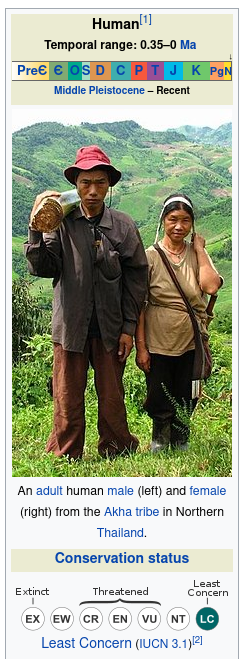
\includegraphics[height=0.75\textheight]{images/human}
            \newline
            {\tiny Source: wikipedia.org}
        \end{center}

\end{columns}
\end{frame}


\begin{frame}{The Solution}
    \begin{itemize}[<+->]
        \item The most important skill in programming is
            decomposition.
        \item That is, the key skill is the ability to break a 
            problem down into smaller chunks.
        \item Because we are violent ape-brained creatures, we have
            to have mechanisms which allow us to focus on smaller
            parts of a programming function.
        \item C++ provides two such mechanisms:
            \begin{itemize}
                \item Modular Decomposition (functions)
                \item Object Oriented Programming (classes and
                    objects)
            \end{itemize}
        \item These allow us to create abstractions.
        \item We have to hide the other 4,393 parts of the problem so
            we can focus on the seven parts we are capable of.
    \end{itemize}
\end{frame}

\section{Functions}

\begin{frame}[fragile]{Function Definition}
    \begin{block}{Function Syntax}
        \texttt{\textit{return\_type} \textit{name}( \textit{parameters} )}
        \newline\texttt{\{}
        \newline\verb!    //function body!
        \newline\texttt{\}}
    \end{block}

    \begin{itemize}[<+(2)->]
        \item A function is a block of code that can be called
            multiple times. 
        \item A function's signature consists of the following:
        \begin{description}
            \item[return type] This is the type of value the function
                evaluates to when it is used in an expression.
            \item[name] The identifier which names the function.
            \item[parameters] The local variables which receive the
                arguments of the function.
        \end{description}
    \end{itemize}
\end{frame}

\begin{frame}[fragile]{Example: The Main Function}
    \begin{verbatim}
int main()
{
    cout << "Hello, world" << endl;

    return 0;
}
    \end{verbatim}
    \begin{itemize}[<+->]
        \item Every C++ program has at least one function.
        \item This function is named \texttt{main}.
        \item The \texttt{main} function above takes no arguments.
        \item The \texttt{main} function returns an integer.
        \item We can explicitly return a value by using the
            \texttt{return} keyword.
    \end{itemize}
\end{frame}

\begin{frame}[fragile]{Void Functions}
    \begin{itemize}[<+->]
        \item Sometimes, it is desirable to have a function do
            something, but return no value. 
        \item Such a function has a return type of \texttt{void}
        \item Take a look at \texttt{examples/10-Elephant/roman.cpp}
    \end{itemize}
    \pause
    \begin{adjustbox}{max width=0.9\textwidth, max totalheight=0.63\textheight}
    \begin{BVerbatim}
//Print the roman numeral for the given value.
//This function can print values for 1,4,5,9,and 10
//All other values print "invalid"
void print_roman_numeral(int value) 
{
    if(value == 1) {
        cout << "I";
    } else if(value == 4) {
        cout << "IV";
    } else if(value == 5) {
        cout << "V";
    } else if(value == 9) {
        cout << "IX";
    } else if(value == 10) {
        cout << "X";
    } else {
        cout << "Invalid";
    }
}
    \end{BVerbatim}
    \end{adjustbox}
\end{frame}

\begin{frame}[fragile]{Calling Functions}
    \begin{itemize}[<+->]
        \item Functions are called by typing their name and putting
            their arguments in parenthesis.
        \item Take, for example, the main function from
            \texttt{roman.cpp}
    \end{itemize}
    \pause
    \begin{BVerbatim}
int main()
{
    int x;

    //get the number
    cout << "Enter a number: ";
    cin >> x;

    //print it as a roman numeral
    print_roman_numeral(x);
    cout << endl;
}
    \end{BVerbatim}
\end{frame}

\begin{frame}{The Structure of \texttt{roman.cpp}}
    \begin{itemize}[<+->]
        \item \texttt{roman.cpp} works, but the main function is at
            the end.
        \item It would make more sense to have the main function be
            the first function in the file.
        \item Copy \texttt{roman.cpp} to \texttt{labs/week6}
        \item Try moving the \texttt{print\_roman\_numeral} function
            definition to the end of the file.
        \item Compile and run.  
        \item Why doesn't it work?
    \end{itemize}
\end{frame}

\begin{frame}[fragile]{Function Prototypes}
    \begin{itemize}[<+->]
        \item Function prototypes allow you to declare a function
            before it is defined.
        \item This is a sort of ``contract'' between you and the
            compiler.
        \item This allows you to have functions in any order in the
            file.  
        \item Change the first few lines of \texttt{roman.cpp} so it
            reads as follows:
            \newline
            \newline
            \begin{BVerbatim}
#include <iostream>

using namespace std;

//function prototypes
void print_roman_numeral(int value);
            \end{BVerbatim}
    \end{itemize}
\end{frame}

\begin{frame}{Best Practice for Files With Functions}
    \begin{itemize}[<+->]
        \item The \texttt{main} function should be the first function
            definition in the file.
        \item You should provide prototypes for every function other
            than the main function.
        \item Your files should be ordered as follows:
        \begin{enumerate}
            \item Opening comment, explaining the program.
            \item All of your \texttt{\#include} directives.
            \item A section for function prototypes. (labeled)
            \item The \texttt{main} function.
            \item All of the other functions.
        \end{enumerate}
        \item Every function (other than \texttt{main}) should have
            a comment before their definition which explains what the
            function does.
    \end{itemize}
\end{frame}

\begin{frame}{Lab Activity: Finish \texttt{print\_roman\_numeral}}
    Edit the \texttt{print\_roman\_numeral} function to include all
    other roman numerals.

    \begin{columns}
    \column{0.33\textwidth}
    \begin{description}
        \item[I] 1
        \item[IV] 4
        \item[V] 5
        \item[IX] 9
        \item[X] 10
    \end{description}
    \column{0.33\textwidth}
    \begin{description}
        \item[XL] 40
        \item[L] 50
        \item[XC] 90
        \item[C] 100
    \end{description}
    \column{0.33\textwidth}
    \begin{description}
        \item[CD] 400
        \item[D] 500
        \item[CM] 900
        \item[M] 1000
    \end{description}
    \end{columns}
\end{frame}

\section{Thinking in Functions}

\begin{frame}[fragile]{Top-Down Design}
    \begin{itemize}[<+->]
        \item As we design a task, we often have tasks that will have
        many sub steps. 
        \item For example:
        \begin{enumerate}
            \item Read a number
            \item Translate into a roman numeral
        \end{enumerate}
        \item We could translate into the following (go ahead and
        change your main function to this):
        \newline
        \begin{adjustbox}{max totalheight=3.8cm}
        \begin{BVerbatim}
int main()
{
    int num;

    //read number
    cout << "Enter a number: ";
    cin >> num;

    indian_to_roman(num);
}
        \end{BVerbatim}
        \end{adjustbox}
    \end{itemize}
\end{frame}

\begin{frame}[fragile]{Lab Activity: Roman Numeral Translator}
    \begin{itemize}[<+->]
        \item Go ahead and add a function prototype for our new
            function:
            \newline\verb!void indian_to_roman(int num);!
        \item Now, at the bottom of your file, add an empty definition
            for the function:
            \newline
            \begin{BVerbatim}
void indian_to_roman(int num) 
{

}
            \end{BVerbatim}
    \end{itemize}
\end{frame}

\begin{frame}{Roman Numeral Translation Steps}
    \begin{itemize}[<+->]
        \item We will translate to roman numerals as follows:
        \begin{enumerate}
            \item Start the value at 1000.
            \item Divide the number by the value.
            \item Print that many of \texttt{print\_roman\_numeral(value)}
            \item Set value to the next roman numeral value.
            \item Subtract what we have just printed from the number.
            \item Repeat the process until the number is zero.
        \end{enumerate}

        \item Let's discuss.  What functions are there in the above?
        \item How do we do each step?
        \item Let's build this thing!
    \end{itemize}
\end{frame}

\begin{frame}{Lab Week 6 Requirements}
    You must have the following for full credit:
    \begin{itemize}
        \item \texttt{count2.cpp} (for loop version)
        \item \texttt{fahrenheit.cpp} (for loop version)
        \item \texttt{double-count.cpp} (fully corrected version)
        \item \texttt{roman.cpp} (able to translate to roman numerals)
    \end{itemize}
\end{frame}


\end{document}


